\subsection{\href{http://www.seconsat.com}{Seconsat}}
   \hypertarget{subsec:seconsat}
In addition to consulting tasks, a wireless device was developed to report temperature, humidity, speed, and other parameters from the box of a cargo truck to a GSM tracking equipment.\\
I've used 0402 technology in a 4-layer PCB with radiofrequency requirements from 200 MHz to 2.4 GHz.\\
I've developed the schematic, and the PCB in Orcad Allegro as shown in the figure \ref{fig:seconsat}.\\
   \begin{figure}
      \begin{center}
         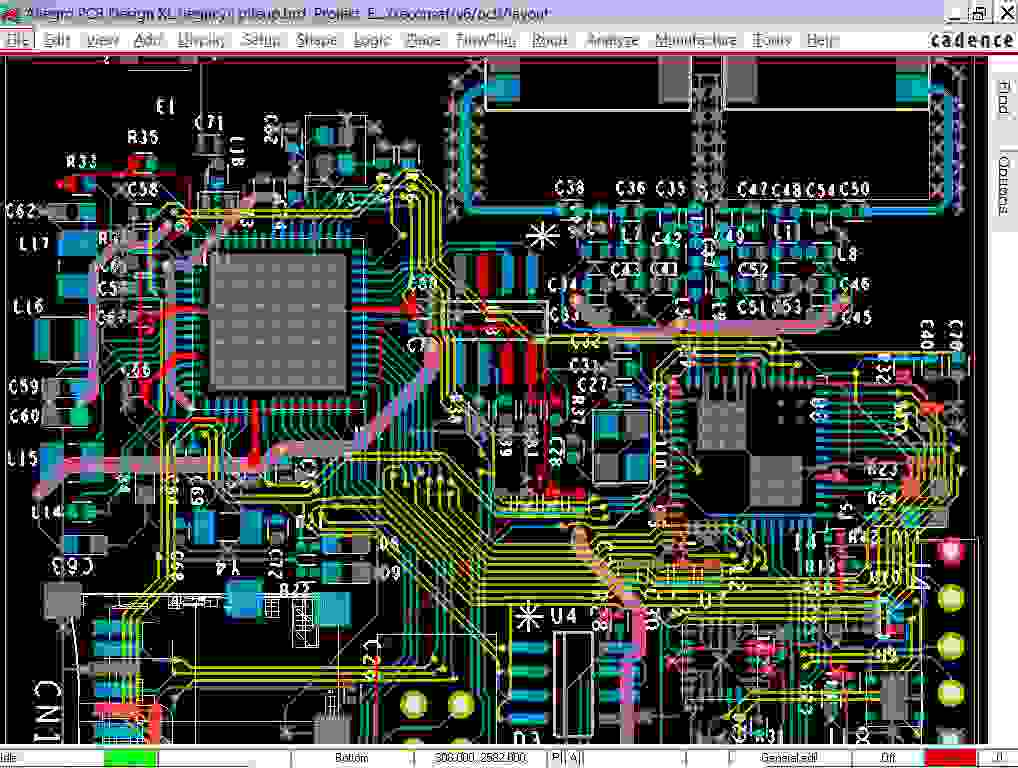
\includegraphics[width=0.49\textwidth]{seconsat1.jpg}
         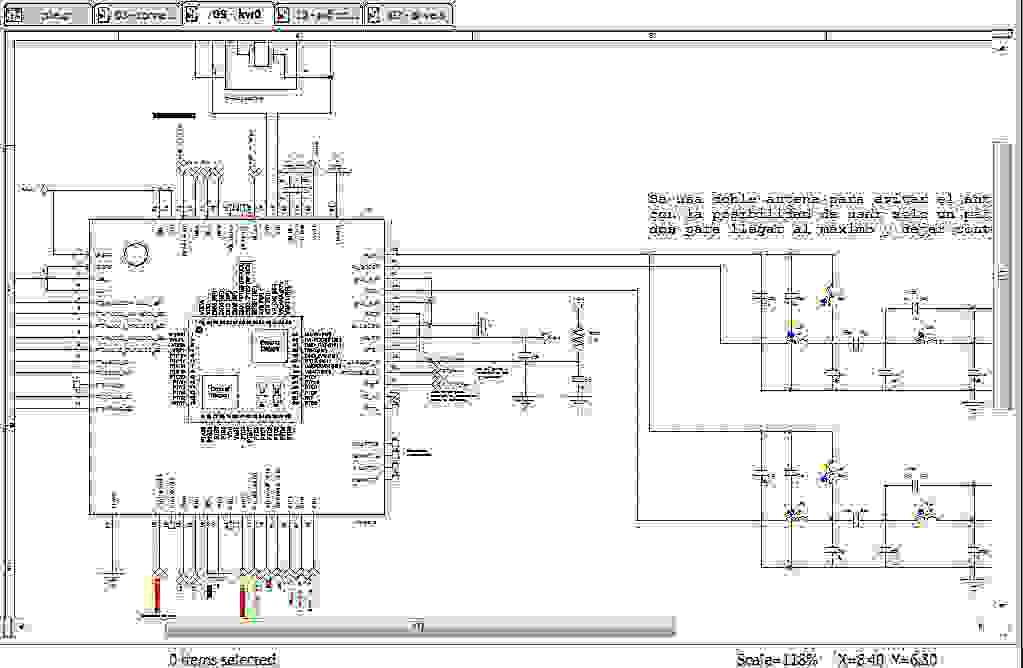
\includegraphics[width=0.49\textwidth]{seconsat2.jpg}
      \end{center}
      \caption{PCB development using one 2.4Ghz and one sub-1Ghz radio for wireless communication.}
      \label{fig:seconsat}
   \end{figure}

